\subsection*{Problema 03}
\textbf{Enunciado:} Calcular la integral indefinida
\begin{align*}
\int \dfrac{\tan x \, dx}{1 + \cos x}
\end{align*}

\textbf{Solución:}
Primero, expresamos la función tangente en términos de seno y coseno usando la identidad trigonométrica $\tan x = \dfrac{\sin x}{\cos x}$:
\begin{align*}
I &= \int \dfrac{\left(\dfrac{\sin x}{\cos x}\right) dx}{1 + \cos x} \\
I &= \int \dfrac{\sin x \, dx}{\cos x (1 + \cos x)}
\end{align*}

Aplicamos el método de sustitución sugerido. Sea $u = \cos x$, de donde el diferencial es $du = -\sin x \, dx$, lo que implica que $\sin x \, dx = -du$. Sustituyendo en la integral:
\begin{align*}
I &= \int \dfrac{-du}{u (1 + u)} \\
I &= -\int \dfrac{du}{u (1 + u)}
\end{align*}

Utilizamos fracciones parciales para descomponer el integrando:
\begin{align*}
\dfrac{1}{u(1 + u)} &= \dfrac{A}{u} + \dfrac{B}{1 + u} \\
1 &= A(1 + u) + Bu
\end{align*}

Evaluando para $u = 0$, obtenemos $A = 1$. Evaluando para $u = -1$, obtenemos $B = -1$. Por lo tanto, la descomposición es:
\begin{align*}
\dfrac{1}{u(1 + u)} &= \dfrac{1}{u} - \dfrac{1}{1 + u}
\end{align*}

Sustituimos esto de vuelta en nuestra integral:
\begin{align*}
I &= -\int \left( \dfrac{1}{u} - \dfrac{1}{1 + u} \right) du \\
I &= -\left( \ln|u| - \ln|1 + u| \right) + C \\
I &= \ln|1 + u| - \ln|u| + C \\
I &= \ln\left| \dfrac{1 + u}{u} \right| + C
\end{align*}

Finalmente, regresamos a la variable original $x$ sustituyendo $u = \cos x$:
\begin{align*}
I &= \ln\left| \dfrac{1 + \cos x}{\cos x} \right| + C \\
I &= \ln\left| \dfrac{1}{\cos x} + 1 \right| + C \\
I &= \ln|\sec x + 1| + C
\end{align*}

La solución general de la integral es:
\begin{align*}
\int \dfrac{\tan x \, dx}{1 + \cos x} = \ln|\sec x + 1| + C
\end{align*}

\begin{figure}[H]
	\centering
	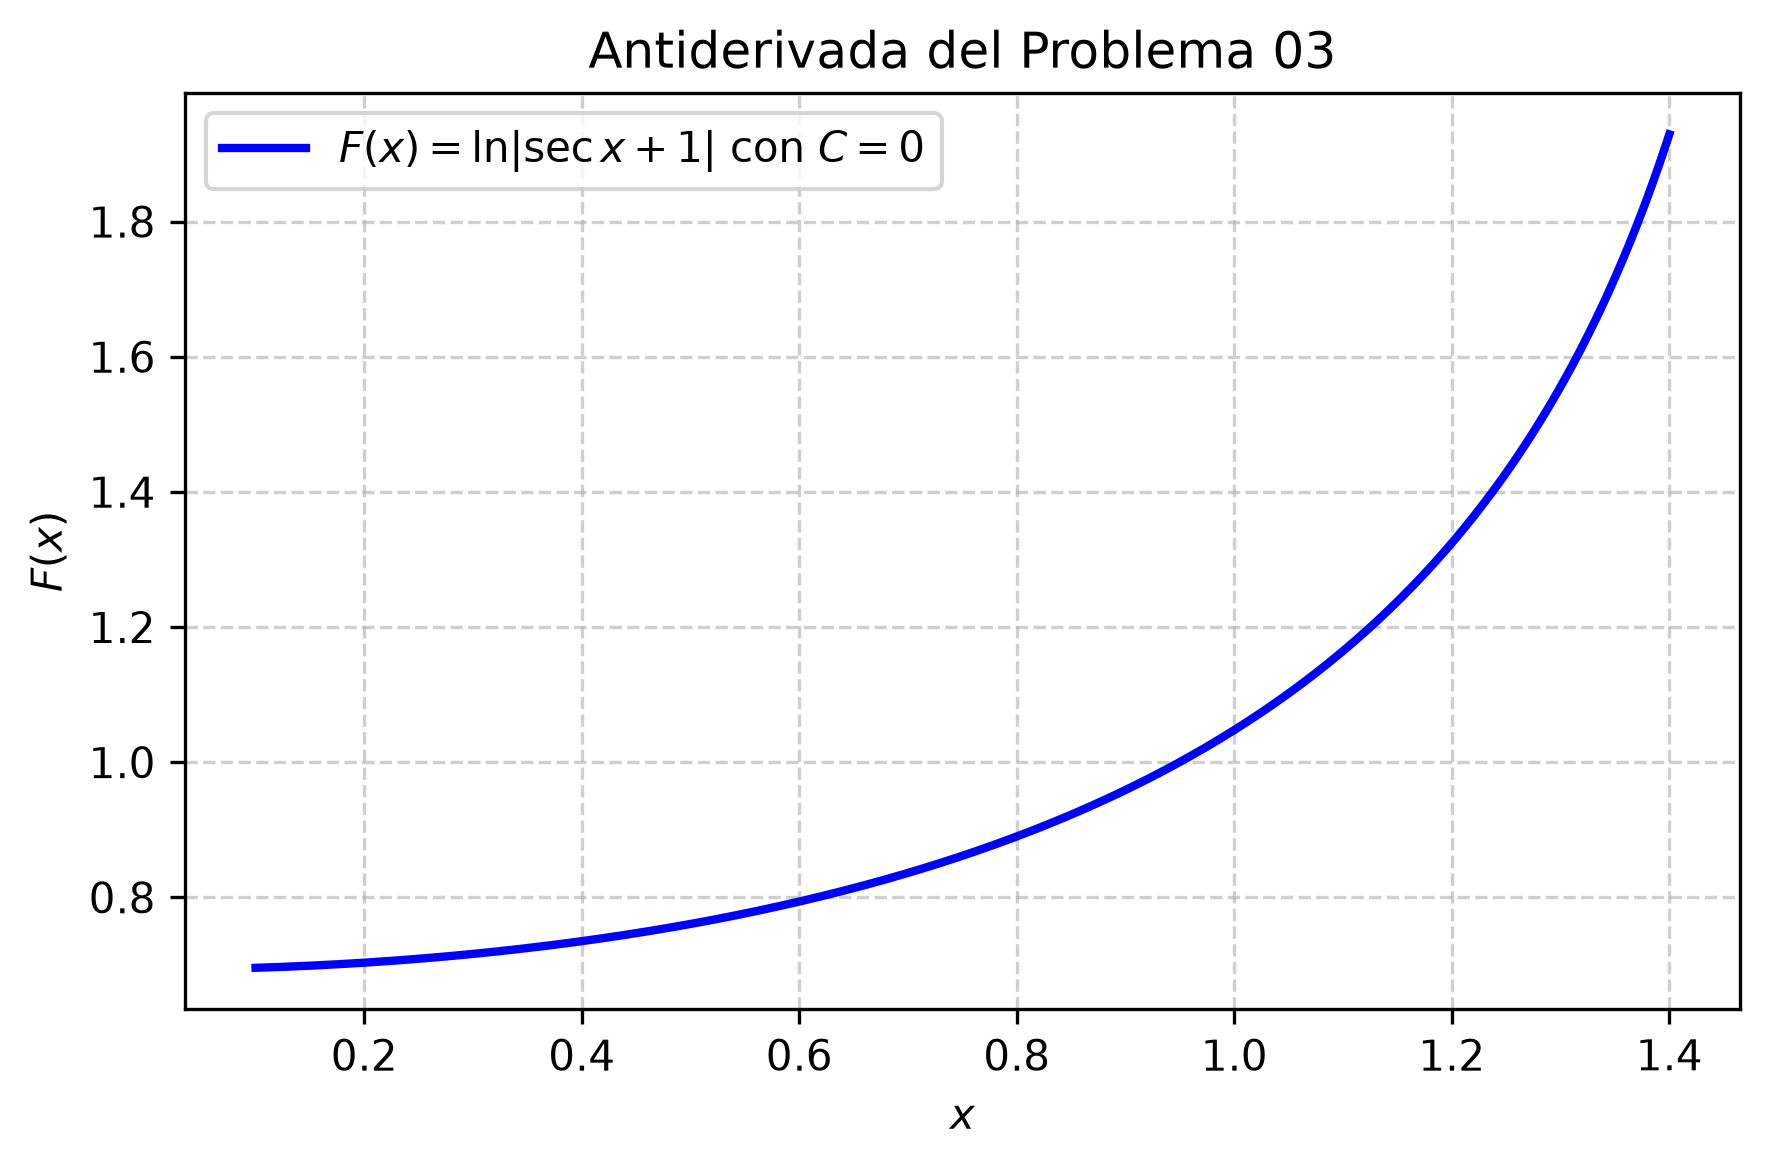
\includegraphics[width=\columnwidth]{semana_04/graficas/SEM04_P03_grafica.png}
	\caption{Representación gráfica de $f(x)$ y su antiderivada $F(x)$ evaluada para la constante de integración $C = 0$ (Problema 03).}
	\label{fig:problema03}
\end{figure}
